\documentclass[conference]{IEEEtran}
\IEEEoverridecommandlockouts
% The preceding line is only needed to identify funding in the first footnote. If that is unneeded, please comment it out.
\usepackage{cite}
\usepackage{amsmath,amssymb,amsfonts}
\usepackage{algorithmic}
\usepackage{graphicx}
\usepackage{textcomp}
\usepackage{xcolor}
\def\BibTeX{{\rm B\kern-.05em{\sc i\kern-.025em b}\kern-.08em
    T\kern-.1667em\lower.7ex\hbox{E}\kern-.125emX}}
\begin{document}

\title{The Research on IoT Botnet
\\
{\rightline{\large-- Use Mirai Botnet as an Example}}
}

\author{\IEEEauthorblockN{Fang Lin}
\IEEEauthorblockA{\textit{Freie Universit\"at Berlin} \\
IoT \& Security Seminar Report
}
}

\maketitle

% Abstract and key words
\begin{abstract}
The Internet of Things (IoT) is becoming an indispensable part of our daily lives, playing an increasingly important role in health, the environment, the family, the military and so on. The Internet of Things has grown tremendously in recent years. However, IoT devices still suffer from basic security vulnerabilities. Hackers use their computing and communication advantages to perform different types of attacks, IoT botnet is one of them. Mirai Botnet is the most typical type of Botnets. This article uses Mirai Bot as the main body of analysis. By analysing the development line, structure and propagation form of Mirai Bot, it analyses how Mirai Bot attacks IoT devices, and analyses how to detect and prevent botnets from technical and non-technical aspects, hoping to gain a deeper understanding of IoT botnets and how to prevent it.
\end{abstract}

\begin{IEEEkeywords}
IoT, Botnet, Mirai Botnet, DDoS, Deep Learning
\end{IEEEkeywords}

% First Part, introduction
\section{\textbf{Introduction}}
The introduction part mainly introduces the background and significance of the research, some basic concepts, and the structure of this article.

\subsection{\textbf{Research Background}}
The IoT botnet is an important reason that makes IoT devices unable to operate normally and leads to network security issues such as the leakage of private information. IoT botnets mainly interfere with the operation of IoT devices by attacking DDoS. Looking back at the history of the IoT botnets invading the IoT devices, a series of network security incidents have occurred in the economic, smart city and so one. As a classic botnet, Mirai botnet is worthy of our in-depth research on botnets to explore the reasons for these things.
\subsection{\textbf{Research Significance}}
On the one hand, through the analysis and research of the Mirai botnet, I can have a deeper understanding of the botnet and also have a better understanding of the security issues of IoT devices. On the other hand, by understanding how to prevent the infringement of botnets, I can also improve my awareness of prevention when using IoT devices, that is, to be able to use IoT devices more sensibly, not to blindly believe and use without them security protection. they, so that the private information can be better protected.
\subsection{\textbf{Basic Concenpts}}
\begin{itemize}
\item \textbf{IoT}\\
he Internet of things (IoT) describes the network of physical objects—a.k.a. "things"—that are embedded with sensors, software, and other technologies for the purpose of connecting and exchanging data with other devices and systems over the Internet.\cite{b16}
\item \textbf{Botnet}\\
A botnet is a
network of infected machines or bots, also called zombies,
that has a command-and-control infrastructure
and is used for various malicious activities such as distributed
denial-of-service (DDoS) attacks.\cite{b10}
\item  \textbf{Mirai Botnet}\\
  The Mirai botnet, composed primarily of embedded
and IoT devices, took the Internet by storm in late 2016
when it overwhelmed several high-profile targets with
massive distributed denial-of-service (DDoS) attacks.\cite{b1}
\item  \textbf{DDoS}\\
In a distributed denial-of-service attack (DDoS attack), the incoming traffic flooding the victim originates from many different sources. This effectively makes it impossible to stop the attack simply by blocking a single source.\cite{b14}
\item  \textbf{Deep Learning}\\
Deep learning (also known as deep structured learning) is part of a broader family of machine learning methods based on artificial neural networks with representation learning. Learning can be supervised, semi-supervised or unsupervised.\cite{b15}
\end{itemize}
\subsection{\textbf{Structure}}
\begin{figure}[htbp]
\centerline{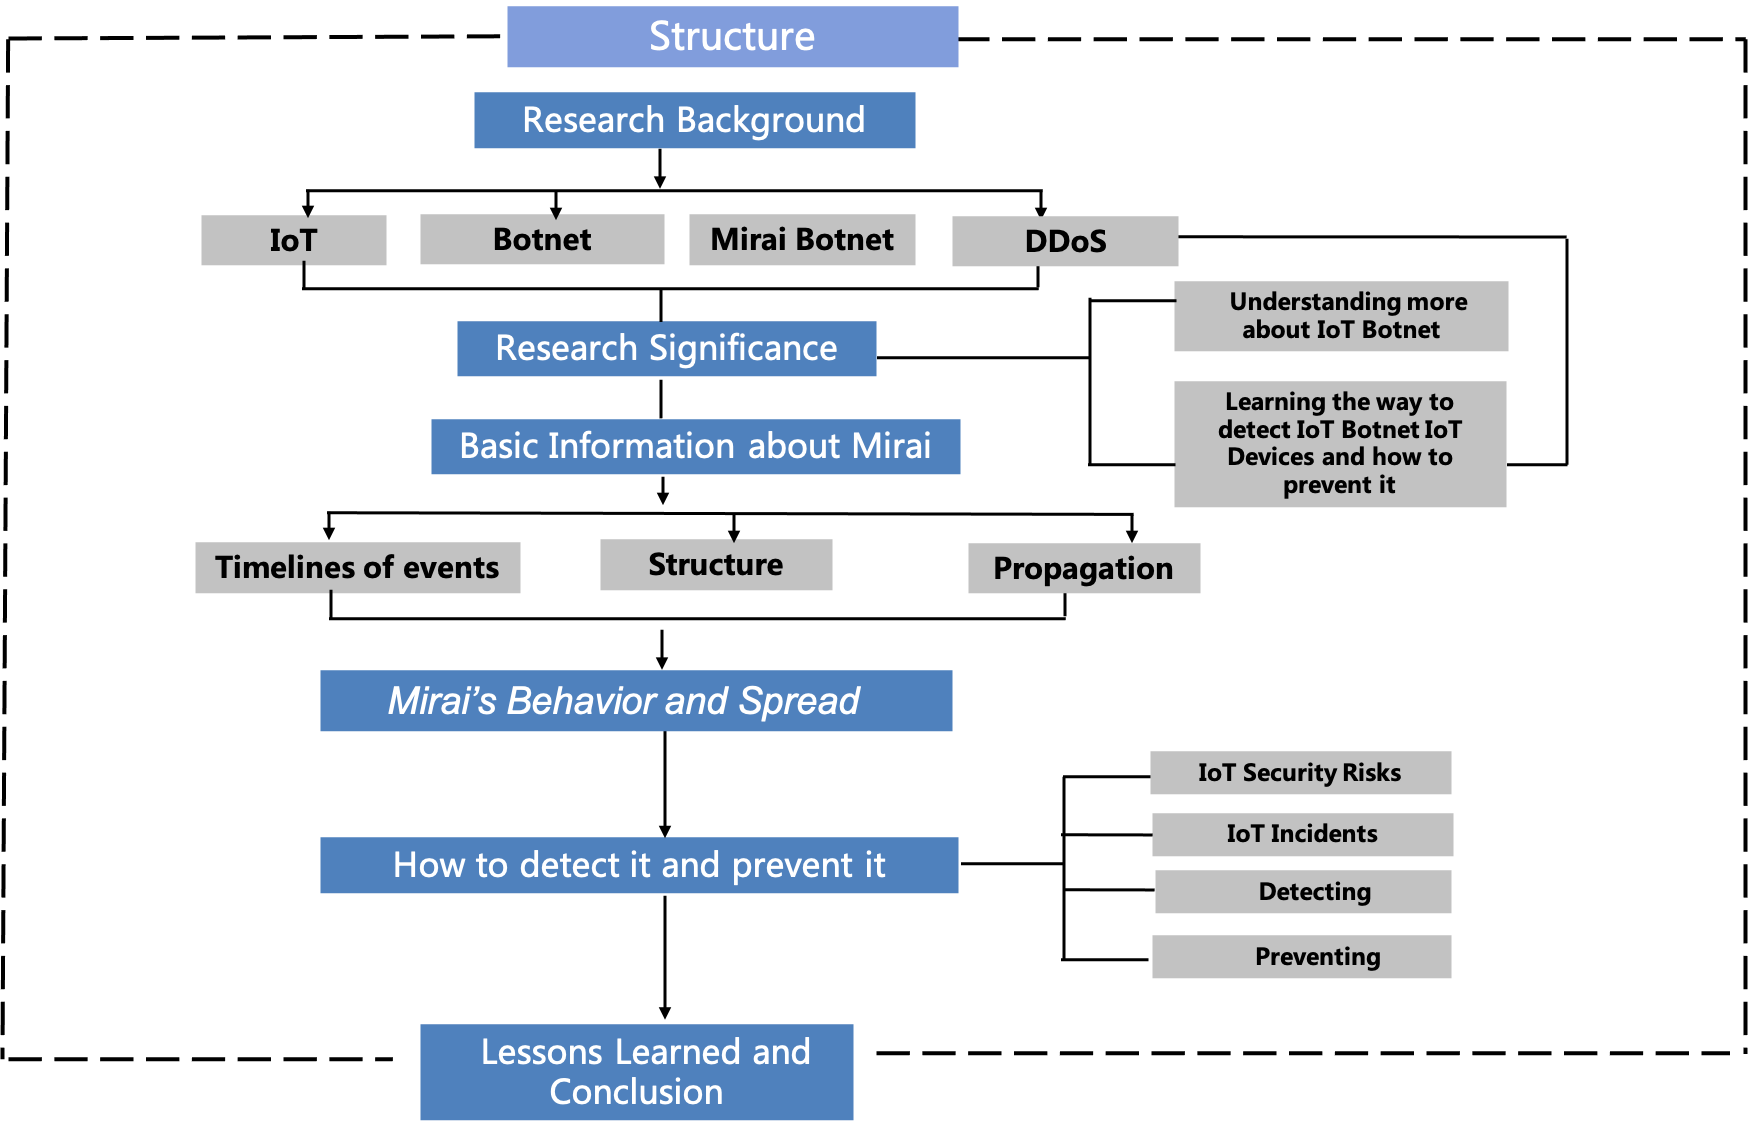
\includegraphics[scale=0.30]{structure.png}}
\caption{Structure of this article}
\label{fig}
\end{figure}

%The second part, introduces Mirai
%\textbf{

\section{\textbf{Basics of IoT Botnets and Mirai Botnet}}
In this section, the basics of IoT botnets and mirai botnet will be introduced. I introduce firstly the basics of IoT Botnets, and then I will mainly write the information of Mirai Botnet, including the timeline of events, the structure and the way of propagation. At the end I will introduce some other botnets and make a small conclusion about the relationships between them.
% General Introduction of a Botnet
\subsection{\textbf{Basics of an IoT Botnet}}
\begin{figure}[htbp]
\flushleft{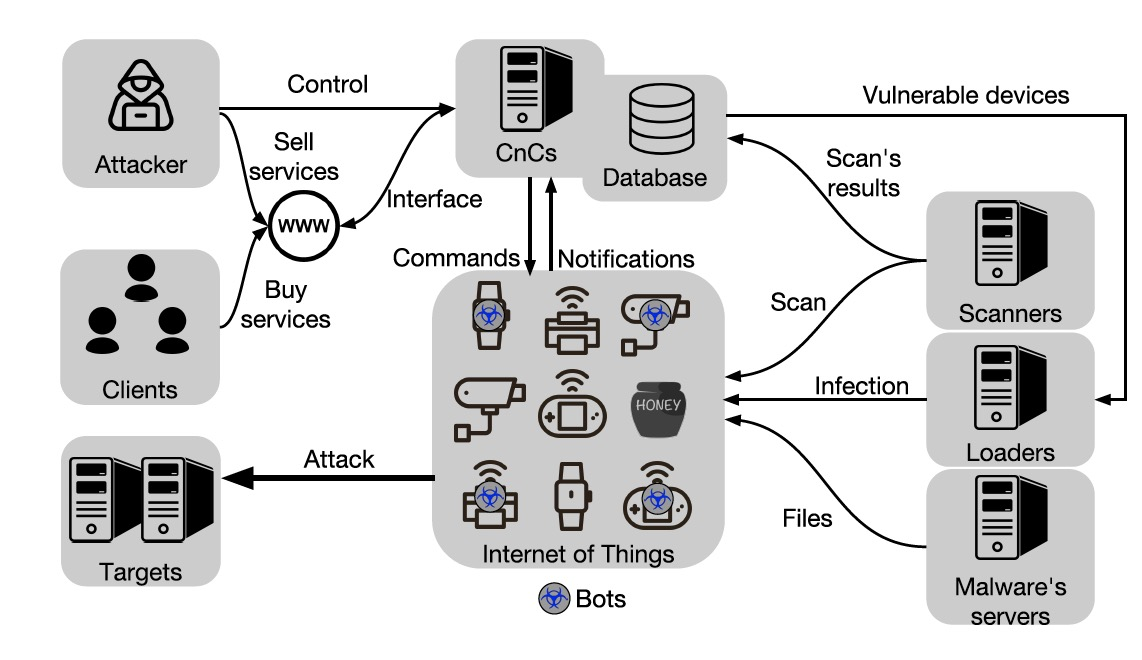
\includegraphics[scale=0.23]{overview.png}}
\caption{Overview of an IoT Botnet\cite{b3}}
\label{fig}
\end{figure}

\begin{itemize}
\item {The left part includes attackers, clients, and targets which are easy to understand. }
\begin{itemize}
\item {Attackers}\\
Attackers are those who try to attack the IoT devices to gain profits.

\item {Clients}\\
Clients are the groups who bought IoT devices and use them as a part of normal life, in the context they are also the victims.
\item {Targets}\\
Targets are the IoT devices which suffered from the attacks from the attackers and then the information of the clients may be exposed.
\end{itemize}
\item {The center  part includes three domains, which are CnCs, Database and Bots, these should be explained more detailed in the following.}
\begin{itemize}
\item {CnCs }\\
Command and control servers (C\&C) are the operators’
interface to the botnet. C\&Cs receive commands
from operators and maintain connections with infected
devices to broadcast commands.\cite{b3}}
\item {Database}\\
Database (potentially distributed) stores information collected
by the botnet, e.g., active bots and scan results.\cite{b3}}
\item {Bots }\\
Bots are infected devices that are part of the botnet.
Bots report their state to C\&Cs and execute the received
commands.\cite{b3}}
\end{itemize}

\item {In the right part there are scanners, loaders and malware's servers.}
\begin{itemize}
\item {Scanners}\\
Scanners probe devices to find telnet and SSH servers to
attempt login and identify vulnerable devices.\cite{b3}}

\item {Loaders}\\
Loaders login to vulnerable devices to download and run
the botnet malware, creating a new bot.\cite{b3}}

\item {Malware's servers}\\
Malware servers host resources used by the botnet such
as shell scripts and executable binaries.\cite{b3}}
\end{itemize}

\item{How IoT devices will be infected?}

\begin{itemize}
\item{ The scanner first identifies vulnerable devices and reports to the central database.}
\item{The loader then connects to the vulnerable device to download and run the malware. During the infection process, the loader accesses the server to download and run the malware binary file on the vulnerable device. }
\item{Once infected, the bot will connect to the C\&C of the botnet and wait for commands. To prevent subsequent infection attempts from other botnets, the IoT botnet disables the telnet and SSH services of the infected device. }
\item{Finally, operators may sell botnet services (for example, denial of service attacks), which are usually accessible through the client’s web interface }

\end{itemize}
\end{itemize}

%Timeline of events
\subsection{\textbf{The Timeline of Mirai Botnet }}

\begin{figure}[htbp]
%\flushright
\flushright{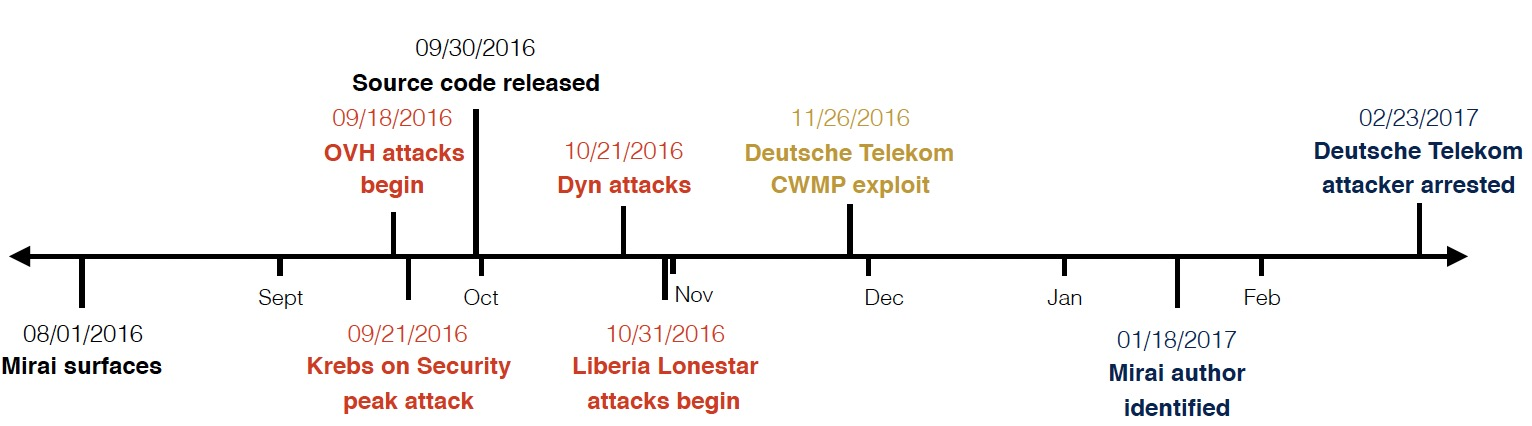
\includegraphics[scale=0.18]{timeline.png}}
\caption{Timeline of events: Major attacks (red), exploits (yellow), and events (black) related to the Mirai botnet.\cite{b1}}
\label{fig}
\end{figure}
From Figure 3\cite{b1}, we can see that on August 1, 2016, Mirai’s surfaces were released. Mirai’s first attack was on September 18, 2016, which was OVH attacks. On the 21st, it attacked DNS provider Dyn. During the two attacks, the source code was released on the Internet. At the end of November, it exploited the vulnerability of Deutsche Telekom CWMP. On January 18, 2017, the author of Mirai was confirmed and arrested at the end of February of the same year.

\subsection{\textbf{The Structure and Propagation of Mirai Botnet}}
This chapter introduces the structure and propagation of Mirai Botnet mainly by figure 4\cite{b1}, which basically follows the structure of an Iot Botnet, but will be more specific and orientational just about Mirai Botnet.

\begin{figure}[htbp]
\flushleft{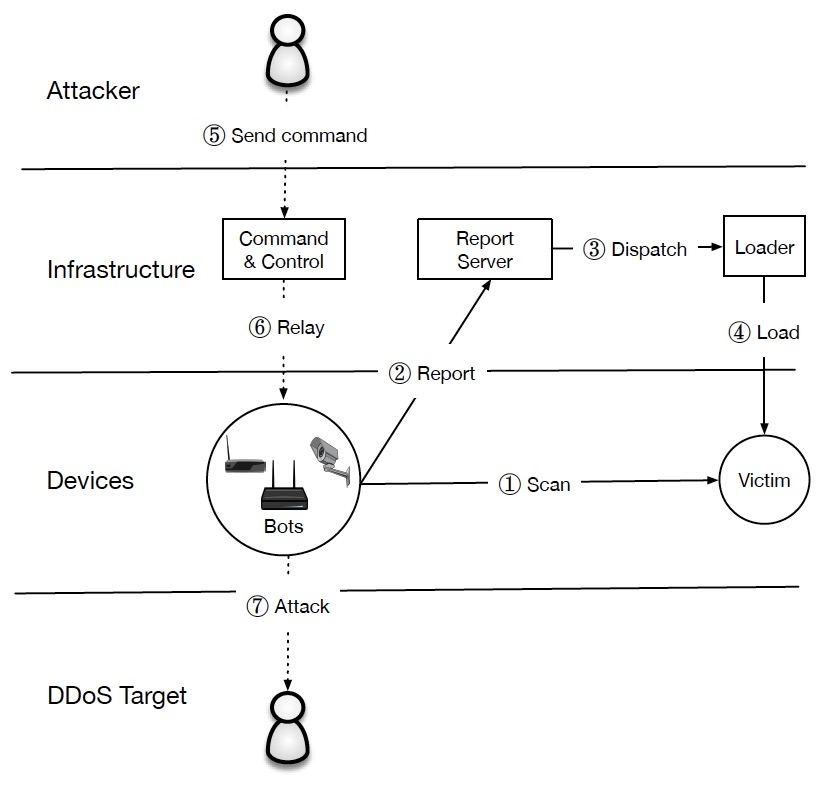
\includegraphics[scale=0.3]{mirai.png}}
\caption{\textbf{Mirai Operation}—Mirai bots scan the IPv4 address
space for devices that run telnet or SSH, and attempt to log in using
a hardcoded dictionary of IoT credentials. Once successful,
the bot sends the victim IP address and associated credentials to
a report server, which asynchronously triggers a loader to infect
the device. Infected hosts scan for additional victims and accept
DDoS commands from a command and control (C2) server.\cite{b1}}
\label{fig}
\end{figure}

\paragraph{\textbf{The Structure  of Mirai Botnet}}\\

Compare to figure 2,  the components of the structure of  Mirai Botnet are almost the same, except there is a report server of mirai botnet structure.
\textbf{Report Server} is a server which Bots will report the victim IP address to it.
In the figure 4\cite{b1}, four layers are designed to describe the mirai botnet structure.

\begin{itemize}
\item{ \textbf{Attacker}}\\
The same as in figure 2, it's the hackers who want to attack the IoT devices.
\item{\textbf{Infrastructure}}\\
In Infrastructure Layer, there are three components, C\&C, Roport Server and Loader.
\item{\textbf{Devices}}\\
The Devices layer is made of bots and victim, the victim here is the victim IoT device.
\item{\textbf{DDoS Targer}}\\
Easy to understand, it's the clients of an IoT devices, which their devices are attacked by Mirai Botnet.

\end{itemize}
\paragraph{\textbf{The Propagation of Mirai Botnet}}\\
As we can see in figure 4, there are 7 phases about the propagation of Mirai Botnet.



\begin{itemize}
\item{ \textbf{Phase 1}}\\
Mirai spread by first entering
a rapid scanning phase 1 where it asynchronously and
“statelessly” sent TCP SYN probes to pseudorandom IPv4
addresses, excluding those in a hard-coded IP blacklist, on
Telnet TCP ports 23 and 2323 (hereafter denoted TCP/23
and TCP/2323). If Mirai identifies a potential victim, it entered
into a brute-force login phase in which it attempted
to establish a Telnet connection using 10 username and
password pairs selected randomly from a pre-configured
list of 62 credentials.\cite{b1}
\item{ \textbf{Phase 2}}\\
At the first successful login, Mirai
sent the victim IP and associated credentials to a hardcoded
report server.
\item{ \textbf{Phase 3}\\
A separate loader program asynchronously infected
these vulnerable devices by logging in, determining
the underlying system environment.
\item{ \textbf{Phase 4}}\\
And at the end  this separate loader program infected the devices by downloading
and executing architecture-specific malware.

\item{ \textbf{Phase 5}}\\
The attackers will send the command to C\&C services.
\item{ \textbf{Phase 6}}\\
 The C\&C services relay the instruction from the attacker to certain bots.

\item{ \textbf{Phase 7}}\\
At the end, the bots will attack the DDoS Target.
\\

\item{ After a successful infection, Mirai attempted to conceal
its presence by deleting the downloaded binary and obfuscating
its process name in a pseudorandom alphanumeric
string. As a consequence, Mirai infections did not
persist across system reboots. In order to fortify itself,
the malware additionally killed other processes bound
to TCP/22 or TCP/23, as well as processes associated
with competing infections. At this point, the bot listened for attack commands from the command and control
server (C2) while simultaneously scanning for new
victims.\cite{b1}}
\end{itemize}


\subsection{\textbf{Other Botnets}}

In this subsection three other botnets will be shortly introduced.

\begin{itemize}
\item{
\textbf{The first IoT botnet written in the
Lua programming language was reported
by MalwareMustDie in late August
2016.} Most of its army is composed
of cable modems with ARM CPUs
and using Linux. This malware incorporates
sophisticated features such
as an encrypted C&C communication
channel and customized iptables rules
to protect infected devices.\cite{b8}}

\item{
\textbf{The Hajime botnet, discovered in
October 2016 by Rapidity Networks,
uses a method of infection similar to
that of Mirai.} However, rather than having a centralized architecture, Hijame
relies on fully distributed communications
and makes use of the
BitTorrent DHT (distributed hash tag)
protocol for peer discovery and the
uTorrent Transport Protocol for data
exchange. Every message is RC4 encrypted
and signed using public and
private keys. So far, Hajime hasn’t evidenced
malicious behavior; in fact,
it actually closes potential sources
of vulnerabilities in IoT devices that
Mirai- like botnets exploit, causing
some researchers to speculate that it
was created by a whitehat.But its
true purpose remains a mystery.}

\item{
\textbf{A BusyBox-based IoT botnet like
Mirai, BrickerBot was unearthed by
Radware researchers in April 2017.}
By leveraging SSH service default credentials,
misconfigurations, or known
vulnerabilities, this malware attempts
a permanent denial-of-service (PDoS)
attack against IoT devices using various
methods that include defacing
a device’s firmware, erasing all files
from its memory, and reconfiguring
network parameters.}

\item{
\textbf{
Linux/IRCTelnet is a new IRC botnet ELF malware aimed
at IoT devices with IPv6 capabilities. } IRCTelnet combining
the concept of Tsunami for IRC protocol, BASHLITE
for the infection techniques (telnet brute force access and
code injection) and using theMirai botnet’s IoT credential
list. The base source code of LightAidra/Aidra is used to
build the new botnet malware. The botnet is using UDP,
TCP flood along with other series of attack methods in
both IPv4 and IPv6 protocol. The new malware features
the extra IP spoof option in both IPv4 or IPv6.\cite{b2}}

\end{itemize}


%The third part, introduces how Mirai attacks IoT devices
\section{\textbf{ Watching Mirai's Behavior and Tracking Mirai’s Spread}}

In Chapter II I write the basic structure about Mirai Botnet and  I describe the propagation of the Mairi Botnet, it's actually the basic route how Mairi attacks IoT devices.
 In this Chapter I will go further about Mirai Botnet by summarising the analysis from article \cite{b1} in two aspects,  one is by using the network vantage
points: a large, passive network telescope, Internet-wide
scanning, active Telnet honeypots, logs of C2 attack
commands, passive DNS traffic, and logs from DDoS
attack targets to get the information about how Mirai Botnet behavior, another aspect is by tracking Mirai's Spread to know further how it works, and may contribute the our next chapter.
\subsection{\textbf{Mirai's Behavior}}

\paragraph{\textbf{Network Telescope}}\\
Mirai’s indiscriminate, rapid scanning strategy lends itself
to tracking the botnet’s propagation to new hosts. The authors\cite{b1}}
monitored all network requests to a network telescope
composed of 4.7 million IP address operated by Merit
Network over a seven month period from July 18, 2016
to February 28, 2017.

   On average, the network telescope
received 1.1 million packets from 269,000 IP addresses
per minute during this period. To distinguish Mirai traffic
from background radiation and other scanning activity,
we uniquely fingerprinted Mirai probes based on
an artifact of Mirai’s stateless scanning whereby every
probe has a TCP sequence number—normally a random
32-bit integer—equal to the destination IP address. The
likelihood of this occurring incidentally is 1=232, and we
would expect to see roughly 86 packets demonstrating
this pattern in our entire dataset. In stark contrast, we
observed 116.2 billion Mirai probes from 55.4 million IP
addresses. Prior to the emergence of Mirai, we observed
only three IPs that perform scans with this fingerprint.
Two of the IP addresses generated five packets; two on
TCP/80 and three on TCP/1002. The third IP address belongs
to Team Cymru, who conducts regular TCP/443
scans.
\paragraph{\textbf{Active Scanning}}\\
In order to determine the
manufacturer and model of devices infected with Mirai,
the authors \cite{b1} leveraged Censys, which actively scans the IPv4
space and aggregates application layer data about hosts on
the Internet.

A number of challenges make accurate device labeling
difficult. First, Mirai immediately disables common outward
facing services (e.g., HTTP) upon infection, which
prevents infected devices from being scanned. Second,
Censys scans often take more than 24 hours to complete,
during which devices may churn to new IP addresses. Finally,
Censys executes scans for different protocols on
different days, making it difficult to increase label specificity
by combining banners from multiple services. 

A conclusion is that devices with open
services that are not closed by Mirai (e.g., HTTPS and
FTP) can appear repeatedly in Censys banner scans during
our measurement window (due to churn) and thus lead to
over counting when compared across protocols. 
\paragraph{\textbf{Telnet Honeypots}}
In order to track the evolution of Mirai’s capabilities, the authors \cite{b1}  collected
binaries installed on a set of Telnet honeypots that masqueraded
as vulnerable IoT devices. At the end they extracted
the set of logins and passwords, IP blacklists, and C2 domains
from these binaries, identifying 67 C2 domains and
48 distinct username/password dictionaries (containing a
total 371 unique passwords).
\paragraph{\textbf{Passive \& Active DNS}}
Following the public release of Mirai’s source code, competing
Mirai botnet variants came into operation.  the authors \cite{b1}
disambiguated ownership and estimate the relative size
of each Mirai strain by exploring passive and active DNS
data for the 67 C2 domains that we found by reverse engineering
Mirai binaries. We also leveraged our DNS data
to map the IP addresses present in attack commands to
victim domain names. In total,  33 unique DNS
clusters of Mirai Botnet are identified.

\paragraph{\textbf{Attack Commands}}
To track the DDoS attack commands issued by Mirai
operators, Akamai ran a “milker” from September 27,
2016–February 28, 2017 that connected to the C2 servers found in the binaries uploaded to their honeypots. 

The authors \cite{b1}note that a naive analysis of attack
commands overestimates the volume of attacks and targets:
individual C2 servers often repeat the same attack
command in rapid succession, and multiple distinct C2
servers frequently issued the same command. 
\paragraph{\textbf{DDoS Attack Traces}}

For Google Shield, The authors \cite{b1} shared a list of IP addresses
observed by our network telescope and in turn
received aggregate statistics on what fraction matched
any of 158.8K IP addresses involved in a 1-minute Mirai
HTTP-flood attack on September 25, 2016. Finally, Dyn
provided them with a set of 107.5K IP addresses associated
with a Mirai attack on October 21, 2016.

\subsection{\textbf{Tracking Mirai's Spread}}

\paragraph{\textbf{Bootstrapping}}
Mirai’s comparatively modest initial
growth may be due to the low bandwidth and computational
resources of infected devices, a consequence of the
low-accuracy, brute-force login using a small number of
credentials, or simply attributable to a bottleneck in loader
infrastructure.
\paragraph{\textbf{Steady State Size}}
The authors \cite{b1} observed multiple phases in Mirai’s life: an initial
steady state of 200,000–300,000 infections in September
2016; a peak of 600,000 infections at the end of November
2016; and a collapse to roughly 100,000 infections at
the end of our observation window in late February 2017
(Figure 3). Even though hosts were initially compromised
via a simple dictionary attack, Mirai was able to infect
hundreds of thousands of devices. This is similar in scale
to historical botnets such as the prolific Srizbi spam botnet
(400,000 bots ), which was responsible for more
than half of all global botnet spam , and the Carna
botnet (420,000 bots), the first botnet of IoT devices
compromised using default credentials.
\paragraph{\textbf{Global Distribution}}
Where Mirai infections were geographically
concentrated?

\begin{figure}[htbp]
\flushleft{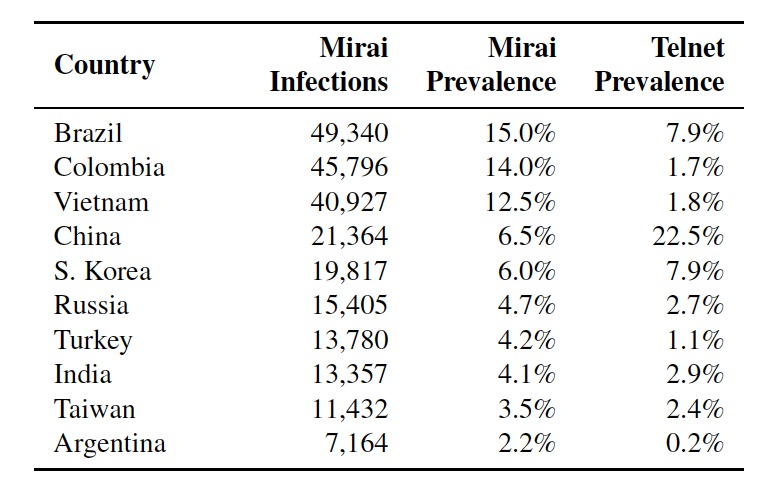
\includegraphics[scale=0.33]{geo.png}}
\caption{Geographic Distributiont\cite{b1}}
\label{fig}
\end{figure}

In figure 5 we can see, most Mirai infections originate from
Located in Brazil (15.0\%), Colombia (14.0\%) and
Vietnam (12.5\%)

\paragraph{\textbf{Device Composition}}

While cursory evidence suggested that Mirai targets IoT
devices—Mirai’s dictionary of default usernames and
passwords included routers, DVRs, and cameras.

After the gathering and analysing of the authors \cite{b1}, the devices they identified were primarily
network-attached storage appliances, home routers, cameras,
DVRs, printers, and TV receivers made by dozens
of different manufacturers.

The manufacturers responsible
for the most infected devices we could identify are:
Dahua, Huawei, ZTE, Cisco, ZyXEL, and MikroTik.

The data indicates that some of the world’s top manufacturers
of consumer electronics lacked sufficient security
practices to mitigate threats like Mirai, and these
manufacturers will play a key part in ameliorating vulnerability.
Unfortunately, as discussed in the previous
section, the menagerie of devices spanned both countries
and legal jurisdictions, exacerbating the challenge of coordinating
technical fixes and promulgating new policy to
safeguard consumers in the future.
\paragraph{\textbf{Device Bandwidth}}
Mirai was primarily powered by devices with limited
computational capacity and/or located in regions with low
bandwidth.

%Fourth Section, how to detect it and prevent it.
\section{\textbf{How to detect and Prevent Mirai Botnet and other Botnets}}


\subsection{\textbf{IoT Security Risks}}
This chapter introduces some basick security risks of IoT so that we know why some attacks are easy to be taken.


\subsection{\textbf{Some Incidents of IoT caused by Botnets }}
I'm not very sure if I should write some certain examples about some events. Above I already mentioned the timeline of events which are concerned with just Mirai Botnet. However, I'm also supposed to provide some examples which are not 
that closely to DDoS, I mean Mirai Botnet is obviously a DDoS attacking Botnet. Somehow I think maybe to give some other incidents by not just DDoS attacking attacks maybe help to improve the width of this article.
(So maybe if at the end the words number doesn't satisfy the requirement, this part is then needed. )

\subsection{\textbf{Detecting}}
Here I may use two specific examples by Deep Learning based detection system.
The thing now is that I don't how further I should write about this chapter, since to describe the algorithms and the structure of DL is not very important to this article

\subsection{\textbf{Preventing}}
This Chapter is about some basic techniques that we can use to avoid the attacks from Botnet and also some IoT security strategies which can prevent IoT devices from suffering the attacks from Botnets./
\paragraph{\textbf{Protection Techniques }}
\begin{itemize}
\item{1}
\item{2}
\item{3}
\item{4}
\item{5}
\item{6}
\end{itemize}
\paragraph{\textbf{ IoT Security Strategy }}
\begin{itemize}
\item{1}
\item{2}
\item{3}
\item{4}
\item{5}
\item{6}
\end{itemize}


%Last Section, how to detect it and prevent it.
\section{\textbf{Lessoned Learned and Conclusion}}
\subsection{\textbf{Lessoned Learned }}
\begin{itemize}
\item{1}
\item{2}
\item{3}
\item{4}
\item{5}
\item{6}
\end{itemize}
\subsection{\textbf{Conclusion}}
\begin{itemize}
\item{1}
\item{2}
\item{3}
\item{4}
\item{5}
\item{6}
\end{itemize}



%\section*{References}


%\begin{thebibliography}{00}
%\bibitem{b1} G. Eason, B. Noble, and I. N. Sneddon, ``On certain integrals of Lipschitz-Hankel type involving products of Bessel functions,'' Phil. Trans. Roy. Soc. London, vol. A247, pp. 529--551, April 1955.
%\bibitem{b2} J. Clerk Maxwell, A Treatise on Electricity and Magnetism, 3rd ed., vol. 2. Oxford: Clarendon, 1892, pp.68--73.
%\bibitem{b3} I. S. Jacobs and C. P. Bean, ``Fine particles, thin films and exchange anisotropy,'' in Magnetism, vol. III, G. T. Rado and H. Suhl, Eds. New York: Academic, 1963, pp. 271--350.
%\bibitem{b4} K. Elissa, ``Title of paper if known,'' unpublished.
%\bibitem{b5} R. Nicole, ``Title of paper with only first word capitalized,'' J. Name Stand. Abbrev., in press.
%\bibitem{b6} Y. Yorozu, M. Hirano, K. Oka, and Y. Tagawa, ``Electron spectroscopy studies on magneto-optical media and plastic substrate interface,'' IEEE Transl. J. Magn. Japan, vol. 2, pp. 740--741, August 1987 [Digests 9th Annual Conf. Magnetics Japan, p. 301, 1982].
%\bibitem{b7} M. Young, The Technical Writer's Handbook. Mill Valley, CA: University Science, 1989.
%\end{thebibliography}
%\vspace{12pt}




\begin{thebibliography}{00}
\bibitem{b1}Manos Antonakakis, Georgia Institute of Technology; Tim April, Akamai; Michael Bailey, University of Illinois, Urbana-Champaign; Matt Bernhard, University of Michigan, Ann Arbor; Elie Bursztein, Google; Jaime Cochran, Cloudflare; Zakir Durumeric and J. Alex Halderman, University of Michigan, Ann Arbor; Luca Invernizzi, Google; Michalis Kallitsis, Merit Network, Inc.; Deepak Kumar, University of Illinois, Urbana-Champaign; Chaz Lever, Georgia Institute of Technology; Zane Ma and Joshua Mason, University of Illinois, Urbana-Champaign; Damian Menscher, Google; Chad Seaman, Akamai; Nick Sullivan, Cloudflare; Kurt Thomas, Google; Yi Zhou, University of Illinois, Urbana-Champaign.Understanding the Mirai Botnet. (2017)

\bibitem{b2} Kishore Angrishi. Turning Internet of Things(IoT) into Internet of Vulnerabilities (IoV) : IoT Botnets. (2017)

\bibitem{b3} Artur Marzano, David Alexander, O. Fonseca, E. Fazzion, C. Hoepers, Klaus Steding-Jessen, M. H. P. Chaves, Ítalo S. Cunha, D. Guedes, W. Meira .The Evolution of Bashlite and Mirai IoT Botnets. 2018 IEEE Symposium on Computers and Communications (ISCC) 

\bibitem{b4}Basheer Al-Duwairi, Wafaa Al-Kahla, Mhd Ammar AlRefai, Yazid Abdelqader, Abdullah Rawash, Rana Fahmawi. SIEM-based detection and mitigation of IoT-botnet DDoS attacks. (2019) 

\bibitem{b5}Huy-Trung Nguyen, Quoc-Dung Ngo, Van-Hoang Le. A novel graph-based approach for IoT botnet detection. (2019) 

\bibitem{b6}Stephen Herwig, Katura Harvey, George Hughey, Richard Roberts, Dave Levin. Measurement and Analysis of Hajime, a Peer-to-peer IoT Botnet. (2019) 

\bibitem{b7}Xiaolu Zhang, Oren Upton, Nicole Lang Beebe, Kim-Kwang Raymond Choo. IoT Botnet Forensics: A Comprehensive Digital Forensic Case Study on Mirai Botnet Servers. (2020) 

\bibitem{b8} Constantinos Kolias, George Mason University, Georgios Kambourakis, University of the Aegean Angelos Stavrou, George Mason University Jeffrey Voas, IEEE Fellow. DDoS in the IoT: Mirai and Other Botnets. (2017) 
\bibitem{b9}Priscilla Moriuchi, Sanil Chohan. Mirai-Variant IoT Botnet Used to Target Financial Sector in January 2018. (2018)
\bibitem{b10}Elisa Bertino, Purdue University, Nayeem Islam, Qualcomm. Botnets and Internet of Things Security. (2017) 
\bibitem{b11}Saleh Soltan, Prateek Mittal, and H. Vincent Poor, Princeton University. BlackIoT: IoT Botnet of High Wattage Devices Can Disrupt the Power Grid. (2018) 
\bibitem{b12}Amaal Al Shorman, Hossam Faris, Ibrahim Aljarah. Unsupervised intelligent system based on one class support vector machine and Grey Wolf optimization for IoT botnet detection. (2019) 
\bibitem{b13}Vinayakumar R, Mamoun Alazab Senior Member, IEEE, Sriram S, Quoc-Viet Pham, Soman KP, Simran K. A Visualized Botnet Detection System based Deep Learning for the Internet of Things Networks of Smart Cities. (2020) 
\bibitem{b14}https://en.wikipedia.org/wiki/Denial-of-service\_attack
\bibitem{b15}https://en.wikipedia.org/wiki/Deep\_learning
\bibitem{b16}https://en.wikipedia.org/wiki/Internet\_of\_things
\end{thebibliography}
\vspace{12pt}








\end{document}
